\begin{document}

\maketitle

\section{Sissejuhatus}
\begin{frame}[fragile]
  \frametitle{Eelmine kord}
  Keerulised teemad, rõhk keeruliste süsteemide käitumisel eri olukordades
	\begin{itemize}
		\item Jätkusuutlikkus on oluline teema, kui pealispinna alla vaadata
		\item Muudatused äris on vältimatud, nende tagajärjed ITle mittetriviaalsed
		\item Riskijuhtimine klassikalisel kujul keeruliste süsteemide puhul ei toimi
	\end{itemize}
\end{frame}

\begin{frame}[fragile]
  \frametitle{Täna kavas}
		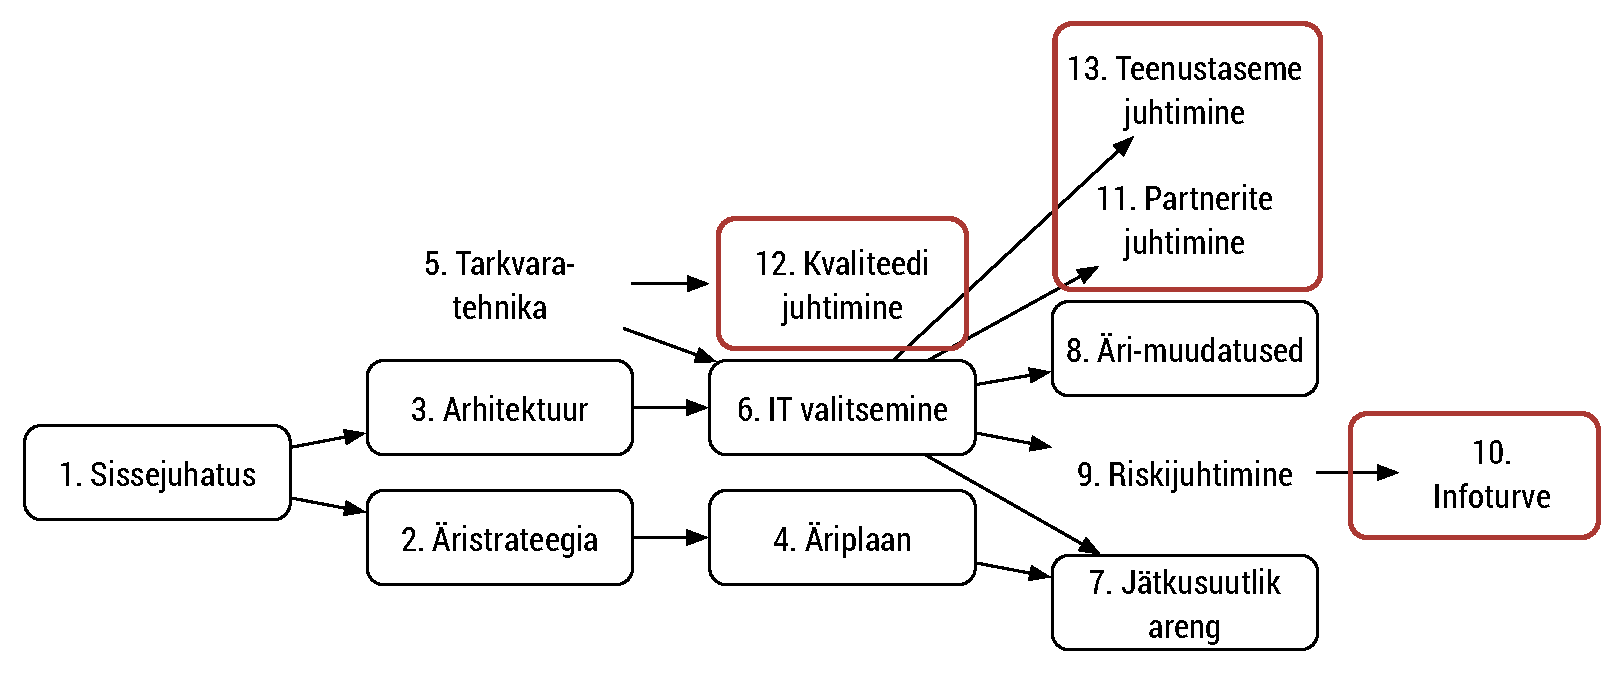
\includegraphics[width=\textwidth]{aine_struktuur_neljas.pdf}
\end{frame}

\section{Infoturve}
\begin{frame}[fragile]
  \frametitle{Küberründe võrratus}
	\begin{center}
	  Rünne tasub end ära siis ja ainult siis, kui:\par
		$S_p>P_f(S_a + P_c S_c)$
	\vfill
	\begin{description}
		\item[$S_p$] Ründest oodatav kasu
		\item[$P_f$] Ründe ebaõnnestumise tõenäosus
		\note{Ründe ebaõnnestumise tõenäosus on reaalselt alati väiksem kui üks: küsimus ei ole sisse saamises, küsimus on kiiruses, hinnas ja sügavuses. Kui otse rünnatakse, siis ka maha võetakse}
		\item[$S_a$] Ründe läbi viimise kulu
		\item[$P_c$] Vahele jäämise tõenäosus
		\item[$S_c$] Vahele jäämise kulu
	\end{description}
	\end{center}

\end{frame}

\begin{frame}[fragile]
  \frametitle{Muutujate seis}
	\begin{itemize}
		\item $S_p$ kasvab, kuna 
			\begin{itemize}
				\item Andmeid saab kasutada (ka) järgmise rünnakute jaoks (tagasiside) 
				\item Interneti sõltuvus reklaamist ja seega privaatsest infost kasvab
				\item Eksisteerib toimiv andmete ja ründeteenuste must turg
			\end{itemize}
		\item $P_f$ kahaneb, kuna süsteemid lähevad järjest keerulisemaks
		\item $S_a$ on dramaatiliselt langenud, kuna 
			\begin{itemize}
				\item Ründed on paljus automatiseeritud
				\item Eksisteerib toimiv üle võetud arvutite must turg
				\item Toimib tagasiside: mida rohkem arvuteid üle võetakse, seda rohkem arvuteid suudetakse rünnata ja seega ka üle võtta
			\end{itemize}
		\item $P_c$ arenenud riikides kasvab, mujal stabiilne
		\item $S_c$ arenenud riikides kasvab kiiresti (vt. megauploadi juhtum)
	\end{itemize}
	\note{Võrratuse parem pool kasvab, kuna ründed lähevad odavamaks ja efektiivsemaks palju kiiremini, kui kasvab vahele jäämise tõenäosus}
\end{frame}


\begin{frame}[fragile]
  \frametitle{Võrratuse järelmid}
	Üksikud intsidendid on asendunud pideva vooga
	\begin{itemize}
		\item Põhjuseks rünnete hinna langemine kiiremini, kui suudetakse tõsta vahele jäämise kulusid
		\item CERT-EE hinnagul ei ole 2015 aasta alguseks enam märgata pause \emph{(spear) phishingu} kampaaniate vahel
		\item Väga suurt rolli mängib automatiseerimine: kuigi automatiseeritud või \emph{drive-by} ründe $P_f$ on suhteliselt suur, on $S_a$ sisuliselt null
	\end{itemize}
\end{frame}

\begin{frame}[fragile]
  \frametitle{Turvalisus ja arhitektuur}
	\begin{center}
		Ohutus (turvalisus) ei ole mitte süsteemi funktsioon vaid selle emergentne käitumine
		\note{Turvalisust ei saa funktsionaalsete nõuete kaudu väljendada. Saab nõuda teatud testide läbi viimist ja saab püstitada ohutusnõuded, kuid ohutust kui sellist ei saa ei nõuda ega testida.}
	\end{center}
	\cite{leveson2011engineering}
\end{frame}

\begin{frame}[fragile]
  \frametitle{Turvalisus tuleb arhitektuurist}
	Turvalisus peab olema sisse ehitatud süsteemi arhitektuuri
	\begin{itemize}
		\item Seda ei saa hiljem lisada ega "külge kruvida"
		\item Kuna me ei suuda emergentsust kontrollida, on turvalisuse tagamine süsteemi elutsüklit läbiv protsess: Ohuanalüüsi tulemid on sisendiks disainiotsustele mis realiseerituna omakorda annavad sisendi uuele ohuanalüüsile
		\item Olulisel kohal on süsteemi kontseptsioon: kas idee on toetuda ühe sõlme turvalisusele või on terve süsteem ehitatud vastupidavaks?
		\note{Lõuna-Korea isikukoodi näide\par}
	\end{itemize}
\end{frame}

\begin{frame}[fragile]
  \frametitle{Infoturbe strateegiast}
	Mõned infoturbe strateegilised aspektid:
	\begin{itemize}
		\item Oluline on määratleda (ja kommunikeerida) aktsepteeritud riskitase
		\begin{itemize}
			\item Kuigi nuga on ohtlik, on ta meil siiski enamasti olemas
			\note{Kasulikkus kompenseerib riski\par}
			\item Järelikult peab olema paigas (kommunikatsiooni) plaan riski realiseerumise puhuks
		\end{itemize}
		\item Strateegiline roll on kogukonnal:
		\begin{itemize}
			\item Süsteemi olulised komponendid ei ole tingimata teie kontrolli all
			\item Tundliku info jagamise aluseks on usaldus
			\note{õige käitumise aluseks on õigeaegne info\par}
			\item Internet on liiga terviklik süsteem, et võiks üksi asju ajada
			\note{Seepärast CERTide võrk tekkiski\par}
			\item Panustage ja te saate vastu
			\note{küberkaitseliit ja muud kogukondlikud ettevõtmised. Selle eelduseks on, et teil on inimesed, kes on suutelised reaalselt panustama\par}
		\end{itemize}

	\end{itemize}
\end{frame}


%Arutelu koht
\begin{frame}[fragile]
  \frametitle{Arutelu koht}
		\begin{center}
			\textbf{Kuidas tellida turvalist tarkvara?}
		\end{center}
\end{frame}


\section{Partnerite juhtimine}
\begin{frame}[fragile]
  \frametitle{Eetikast}
	\begin{center}
		Enne igasugust partneritega tegelemist veendu, et võtmeisikute arusaam eetikast kattub ning mahub mugavalt seaduse raamesse 
		\note{Kohtumine julgeolukuorganitega on pehmelt öeldes ebameeldiv ka siis, kui sa õigeks jääd. Ja kriminaalasi kindlasti mitte ei kiirenda tarkvara valmimist. Eetika pinnalt tekkinud väärtuskonflikt on samuti väga ebameeldiv ja tavaliselt ajakavale hukatuslik.}
	\end{center}
\end{frame}

\begin{frame}[fragile]
  \frametitle{Eesmärkidest}
	\begin{center}
		Teil on partneriga põhimõtteliselt vastuolulised eesmärgid. \par Harjuge ära, ärge võtke isiklikult ja õppige sellega elama
		\note{Oluline on leida ajas piiratud ühine komplekt eesmärke. Partneri motiveerimine.}
	\end{center}
\end{frame}


\begin{frame}[fragile]
  \frametitle{Strateegiline posistioon}
  	Partnerit saab juhtida vaid sobivalt strateegiliselt positsioonilt	
	\begin{itemize}
		\item Tuletage meelde Sun Tzud
		\note{... kes teab, kuidas toimida tugevama ja nõrgema vastasega\par}
		\item Partneril tegeleb reeglina teiega kliendihaldur, kes keskendub vaid teile. Teil on reeglina mitu partnerit
		\note{Tihti on tegemist profiga või nende tiimiga. Hästi makstud oskajad inimesed\par}
		\item Ka väga suured riigid ei suuda enam suurkorporatsioonidele vastu seista \citep{partner}
		\item Ärge tehke endale illusioone oma võimete osas!
		\note{Eestis on vast kaks suuremat panka suutelised suuremaid teenusepakkujaid juhtima}
	\end{itemize}
\end{frame}


\begin{frame}[fragile]
  \frametitle{Strateegiline posistioon}
	\begin{center}
		\begin{quote}
			Therefore the skillful leader subdues the enemy's troops without any fighting
		\end{quote}
	\end{center}
	\cite{tzu2013art}
\end{frame}

\begin{frame}[fragile]
  \frametitle{Toimimisest}
	\begin{center}
		\begin{quote}
	toimi toimimata\\
	ning ei ole nii\\
	et ei oleks juhtimist
   		\end{quote}
	\end{center}
\cite{laozi}
\end{frame}

\begin{frame}[fragile]
  \frametitle{Toimida toimimata}
	\begin{center}
			Kuidas vältida vajadust partnereid juhtida?
			\vfill
			Järgnevas mõned strateegilised võimalused selleks
	\end{center}
	\note{Võib ka vaadata nii, et järgneva abil tekitate endale strateegilise positsiooni}
\end{frame}


\begin{frame}[fragile]
  \frametitle{Tee mittejuhtimiseni}
	\textbf{Ignoreeri kogu probleemi}
	\begin{itemize}
		\item Mis vahet seal on, kes ja kuidas tarnib kohvi ja pastakaid?
		\item Nii te ei saa täpselt seda, mida te tahate
		\note{Aga kohvi puhul reeglina ei ole vahet}
		\item Võib keskenduda ka lihtsalt koostöös parima tulevuse saavutamisele, jättes strateegilised mängud kõrvale
	\end{itemize}
\end{frame}

\begin{frame}[fragile]
  \frametitle{Tee mittejuhtimiseni}
		\textbf{Juhi tehnoloogiat}
	\begin{itemize}
		\item Selle asemel et juhtida partnereid, keskendu oma tehnoloogilise baasi kontrollimisele
		\item Kui kogu IP, arhitektuursed otsused, haldus jne. on teie käes, ei ole palju vahet, kes musta tööd teeb
		\item See kitsendab koostöömudeleid:
		\begin{itemize}
			\item \emph{Time-and-material}
			\item Väga põhjalikult spetsifitseeritud rangelt tehnilised tööd
		\end{itemize}
		\item Mõistlik valik, kontroll tehnoloogia üle on enamasti hea idee
		\item Eeldab tehnilise kompetentsi olemasolu majas
	\end{itemize}
\end{frame}

\begin{frame}[fragile]
  \frametitle{Tee mittejuhtimiseni}
		\textbf{Juhi ja/või kasuta standardeid}
	\begin{itemize}
		\item Selle asemel et juhtida partnereid, kasuta laialt levinud lahtisi standardeid
		\item Vajadusel kirjuta uued
		\item Kui kogu tegevus on standardipõhine, on partneri vahetus suhteliselt lihtne ja valutu
		\item Eriti kasulik kombinatsioonis "jaga ja valitse" strateegiaga
		\item Töömahukas
		\note{Eriti, kui sobivaid standardeid ei ole}
	\end{itemize}
\end{frame}

\begin{frame}[fragile]
  \frametitle{Tee mittejuhtimiseni}
	\textbf{	Juhi kogukonda}
	\begin{itemize}
		\item Ühe partneri juhtimise asemel tekita isereguleeruv seltskond 
		\note{Näiteks open-source kogukond}
		\item Osavalt käima lükatud kogukond hoiab end ise avatuna ja arenemas
		\item Jälle kasulik koos "jaga ja valitse strateegiaga"
		\item Keeruline teha kuid kuldne, kui käima läheb
	\end{itemize}
\end{frame}

\begin{frame}[fragile]
  \frametitle{Strateegilised valikud}
	\textbf{	Jaga ja valitse}
	\begin{itemize}
		\item Jaga oma süsteem rangelt piiritletud komponentideks 
		\item Iga komponent eraldi hanke/hoolduse/uuenduse subjektiks
		\item Piirijoontel kasuta standardeid või rangelt kontrollitud liideseid
		\note{Ka protsessiliidesed (relase!)}
		\item Näiteks: andmehoidla ja rakendusserver on eraldatud S3\footnote{\url{http://aws.amazon.com/s3/}} abil
		\item Hüved:
		\begin{itemize}
			\item Ühelgi partneril ei ole kontrolli terve süsteemi üle
			\item Et liidesed on igal juhul paigas, võib tarnijaid lihtsasti vahetada
			\item Modulariseerimine on igal juhul hea mõte
		\end{itemize}
		\item Vajab tehnilist- ja protsessikompetentsi, töömahukas
	\end{itemize}
\end{frame}


%Arutelu koht
\begin{frame}[fragile]
  \frametitle{Arutelu koht}
		\begin{center}
			\textbf{Kuidas vabaneda end sisse söönud "puugist"?}
		\end{center}
\end{frame}

\begin{frame}[fragile]
  \frametitle{Partnerite juhtimine}
  Kui siiski on vaja partnerit juhtida
	\begin{itemize}
		\item Vali sarnane partner: suurus, ajahorisont, küpsusaste
		\note{Kerry King: Time is not a cool thing to waste\par Olukord, kus sellist saada ei ole, on ohu märk! Miks ei ole see teenus ostetav?}
		\item Käitu kehtestavalt: väljenda oma vajadusi selgelt ja järejekindlalt ning seisa nende eest
		\item Kaasa riskijuhid, partnerid on olulised riskide allikad
		\item Tee selgeks ökosüsteem
		\note{Kes on veel mängijad? Mis on nende huvid? vt. ka märkused seoste kaardistamine kohta\par}
	\end{itemize}
\end{frame}

\begin{frame}[fragile]
  \frametitle{Toimida toimimata}
	\begin{center}
			Isiklik kogemus:\par
			\vfill
			\textbf{Kui partner tundub rumala või pahatahtlikuna,\\ on reeglina põhjust peeglisse vaadata}
			\note{Partnerist lahti saamine on reeglina ressursimahukam kui oma käitumise parandamine}
	\end{center}
\end{frame}

\begin{frame}[fragile]
  \frametitle{Võtmeküsimus}
	\begin{center}
		Kuidas olla pädev klient?
		\note{It takes two to tango!\par Järgnevas levinumad strateegilised valukohad}
	\end{center}
\end{frame}

\begin{frame}[fragile]
  \frametitle{Kontroll IP üle}
  Oluline on saavutada kontroll tekkiva intellektuaalomandi üle
	\begin{itemize}
		\item Omand ei võrdu kontrolliga
		\note{Mu auto on liisingfirma oma aga tööle sõidan sellega mina\par}
		\item Kus tekib intellektuaalomand?
		\begin{itemize}
			\item Ehk: kus tekib väärtus?
			\note{Partnerluse kuldreegel: ära kunagi osta väljast väärtusloomet!\par}
			\item Tänapäeval ei ole tarkvara lähtekood reeglina omaette väärtus 
			\note{Järelikult ei ole kriitiline selle dokumenteerimine. X-tee oli võimalik kuue kuuga nullist uuesti kirjutada\par}
			\item Väga tihti sünnib väärtus kliendi juures
			\note{Teadmine äriprotsessist. Ärianalüütik võib kogu teadmisega minema kõndida!\par}
			\item Küsimus on teadmuses
			\note{Ja seda niisama lihtsalt paberi peal edasi ei anna\par}
		\end{itemize}

	\end{itemize}
	\begin{center}
		\emph{Intellektuaalomandit kontrollib see, \\kes kontrollib seda loovaid inimesi}
		\note{Mida rohkem sinu inimesi on võtmeotsuste juures, seda parem on sinu kontroll}
	\end{center}
		\note{Sest intellektuaalomand tekib IT vallas inimeste peas} 

\end{frame}

\begin{frame}[fragile]
  \frametitle{Kontroll arhitektuuri üle}
  	Oluline on saavutada kontroll süsteemi arhitektuuri üle
	\begin{itemize}
		\item Tuletage meelde arhitektuuri seost ärimudeliga
		\note{Kui te ei kontrolli arhitektuuri, ei kontrolli te oma ärimudelit. Mis on, ütleme, halb\par}
		\item Kontseptsioon on tihedalt seotud väärtuste, mõttemallide ja seeläbi organisatsiooni kultuuriga
		\note{Arhitektuuri kontrollimata lasete te kellegi teise oma organisatsiooni kultuuri mõjutama\par}
		\item Partner lähtub lokaalsest optimumist (või enda omast)
		\note{Teie roll on aga arendada terviklikku süsteemi arhitektuuri\par}
		\item Võõraste väärtuste ja mõttemallide üle võtmine on väga raske. 
		\begin{itemize}
			\item Ka siis, kui need on peidetud arhitektuuri
			\item Vajadus võtta üle tellija mõttemall tasandab mänguvälja
			\note{Aga tõstab hinda! Valikukoht\par}
		\end{itemize}
		\note{Seetõttu ongi arendaja vahetamine reeglina keeruline: igaühel on oma juurdunud viis asju ehitada ja ümber harjumine on keeruline/kallis}
	\end{itemize}
\end{frame}

\begin{frame}[fragile]
  \frametitle{Kontroll suhte üle}
  	Kelle käes on initsiatiiv suhetes partneriga?
	\begin{itemize}
		\item Kõik algab kontrollist lepingu üle
		\begin{itemize}
			\item Iga lepingusse kirjutatud punkt on täitmiseks
			\note{Kunagi ei tohi lepingusse kirjutada asju, mida te "võib olla" jõustate\par}
			\item Kui teie ei suuda lepingut täita, ärge oodake seda ka partnerilt
			\item "Kui me ei täida punkti x, miks peaksime täitma punkti y?"
			\item "Punktis a me tulime ju teile vastu, tulge teie vastu punktis b"
		\end{itemize}
		\item Erilise tähelepanu all olgu suhetele suuantud protsessid, rutiinid, tegevused
		\note{Suhetele suundatud asjade puhul on kriitiline kliendi mõjutamine korrektselt käituma. Vastasel juhul jääte kahe tule vahele: rahul ei ole ei klient ega partner\par}
		\begin{itemize}
			\item Tellimuste esitamine
			\note{Kasutuslugude esitamine nihkub kaks nädalat aga lõpptähtaeg jääb paika. Päriselt või?\par}
			\item Muudatuste juhtimine ja skoobi kontroll
			\item Vastuvõtutestid
			\item Üle andmine ja vastu võtmine
		\end{itemize}
		\item Tuletage meele Sun Tzud
		\note{All warfare is based on deception\par}
		\item \emph{In God we trust, everybody else pays cash}
	\end{itemize}
\end{frame}

%Arutelu koht
\begin{frame}[fragile]
  \frametitle{Arutelu koht}
		\begin{center}
			\textbf{Mida saab teha saamatu kliendiga?}
		\end{center}
\end{frame}

\section{Kvaliteedi juhtimine}

\begin{frame}[fragile]
  \frametitle{Kvaliteedi juhtimine}
	Miks tarkvaras on vead
	\begin{itemize}
		\item Vigade parandamise dünaamiline mudel, selle matemaatiline lahend
		\item Mudeli järelmid: alati on veel vigu, testima tuleb hakata vara
		\item Otsustuskriteeriumid lõpetamiseks: eraldame ratsionaalse ja irratsionaalse. Ratsionnalselt (graafik): kui oleme jõudnud allapoole spetsifikatsiooni veamarginaali
	\end{itemize}
\end{frame}

%Arutelu koht
\begin{frame}[fragile]
  \frametitle{Arutelu koht}
		\begin{center}
			\textbf{4. küsimus}
		\end{center}
\end{frame}

\begin{frame}[fragile]
  \frametitle{Kvaliteedi juhtimine}
	Jaapanlaste lähenemine
	\begin{itemize}
		\item Seos lean liikumisega
		\item Kaizeni olemus
		\item Teede parandamise näide
		\item Selle järeldused tarkvaratehnika ja QA jaoks
	\end{itemize}
\end{frame}

%Arutelu koht
\begin{frame}[fragile]
  \frametitle{Arutelu koht}
		\begin{center}
			\textbf{5. küsimus}
		\end{center}
\end{frame}


\section{Teenustaseme juhtimine}
\begin{frame}[fragile]
  \frametitle{Teenustaseme juhtimine}
	\begin{itemize}
		\item Teenustaseme juhtimise aluseks on teenuse mõiste olemasolu (alignment kõigis kihtides)
		\item Arutelu teenustasemete üle riskijuhtimist kaasamata on lihtsalt grupp jonnivaid inimesi
		\item Teenustase tuleb määratleda läbi riskide
		\item Järelikult tuleb mõõta teenust, mitte masinaid. Masinad, nagu rääkisime, lähevad ennustataval viisil katki
		\item Keerulist süsteemi modelleerima hakka ainult siis, kui sul on palju aega ja raha ning tõsine vajadus. Sest ta on keeruline. Ja, nagu rääkisime, teenustaseme kao põhjus võib olla mõõtmisvea lähedal ja seega raskesti mürast eristatav
	\end{itemize}
\end{frame}


%Arutelu koht
\begin{frame}[fragile]
  \frametitle{Arutelu koht}
		\begin{center}
			\textbf{6. küsimus}
		\end{center}
\end{frame}


\section{Viited}

\begin{frame}[t,allowframebreaks,]
  	\bibliographystyle{plainnat}
	\bibliography{it_strateegia} 

\end{frame}

%\plain{Küsimusi?}
\begin{frame}[plain]
	\begin{center}Küsimusi?\end{center}
\end{frame}


\end{document}